%beamer

% Comment/uncomment this line to toggle handout mode
\newcommand{\handout}{}

%% Beamer-Klasse im korrekten Modus
\ifdefined \handout
\documentclass[handout]{beamer} % Handout mode
\else
\documentclass{beamer}
\fi

%% UTF-8-Encoding
\usepackage[utf8]{inputenc}

\input{../framework/gbi-macros}
\usepackage[blue]{../framework/thwregex}
\usepackage{environ}
\usepackage{bm}
\usepackage{calc}
\usepackage{varwidth}
\usepackage{wasysym}
\usepackage{mathtools}


% Das ist der KIT-Stil
%\usepackage{../TutTexbib/beamerthemekit}
\usepackage[deutsch,titlepage0]{../framework/KIT/beamerthemeKITmod}
\TitleImage[width=\titleimagewd]{../figures/titlepage.jpg}
%\usetheme[deutsch,titlepage0]{KIT}

% Include PDFs
\usepackage{pdfpages}

% Libertine font (Original GBI font)
\usepackage{libertine}
%\renewcommand*\familydefault{\sfdefault}  %% Only if the base font of the document is to be sans serif

% Nicer math symbols
\usepackage{eulervm}
%\usepackage{mathpazo}
\renewcommand\ttdefault{cmtt} % Computer Modern typewriter font, see lecture slides.

\usepackage{csquotes}

%%%%%%

%% Schönere Schriften
\usepackage[TS1,T1]{fontenc}

%% Bibliothek für Graphiken
\usepackage{graphicx}

%% der wird sowieso in jeder Datei gesetzt
\graphicspath{{../figures/}}

%% Anzeigetiefe für Inhaltsverzeichnis: 1 Stufe
\setcounter{tocdepth}{1}

%% Hyperlinks
\usepackage{hyperref}
% I don't know why, but this works and only includes sections and NOT subsections in the pdf-bookmarks.
\hypersetup{bookmarksdepth=subsection} 

%\usepackage{lmodern}
\usepackage{colortbl}
\usepackage[absolute,overlay]{textpos}
\usepackage{listings}
\usepackage{forloop}
%\usepackage{algorithmic} % PseudoCode package 

\usepackage{tikz}
\usetikzlibrary{matrix}
\usetikzlibrary{arrows.meta}
\usetikzlibrary{automata}
\usetikzlibrary{tikzmark}
\usetikzlibrary{positioning}

% Why has no-one come up with this yet? I mean, seriously. -.-
\tikzstyle{loop below right} = [loop, out=-60,in=-30, looseness=7]
\tikzstyle{loop below left} = [loop, out=-150,in=-120, looseness=7]
\tikzstyle{loop above right} = [loop, out=60,in=30, looseness=7]
\tikzstyle{loop above left} = [loop, out=150,in=120, looseness=7]
\tikzstyle{loop right below} = [loop below right]
\tikzstyle{loop left below} = [loop below left]
\tikzstyle{loop right above} = [loop above right]
\tikzstyle{loop left above} = [loop above left]

% Needed for gbi-macros
\usepackage{xspace}

%%%%%%

%% Verbatim
\usepackage{moreverb}

%%%%%%%%%%%%%%%%%%%%%%%%%%%%%%%%%%%% Copy end

%% Tabellen
\usepackage{array}
\usepackage{multicol}
\usepackage{hhline}

%% Bibliotheken für viele mathematische Symbole
\usepackage{amsmath, amsfonts, amssymb}

%% Deutsche Silbentrennung und Beschriftungen
\usepackage[ngerman]{babel}

\usepackage{kbordermatrix}

% kbordermatrix settings
\renewcommand{\kbldelim}{(} % Left delimiter
\renewcommand{\kbrdelim}{)} % Right delimiter

\input{../config.tex}



% define custom \handout command flag if handout mode is toggled  #DirtyAsHellButWell...
\only<beamer:0>{\def\handout{}} %beamer:0 == handout mode

\newcommand{\R}{\mathbb{R}}
\newcommand{\N}{\mathbb{N}}
\newcommand{\Z}{\mathbb{Z}}
\newcommand{\Q}{\mathbb{Q}}
\newcommand{\BB}{\mathbb{B}}
\newcommand{\C}{\mathbb{C}}
\newcommand{\K}{\mathbb{K}}
\newcommand{\G}{\mathbb{G}}
\newcommand{\nullel}{\mathcal{O}}
\newcommand{\einsel}{\mathds{1}}
\newcommand{\Pot}{\mathcal{P}}
\renewcommand{\O}{\text{O}}

\def\word#1{\hbox{\textcolor{blue}{\texttt{#1}}}}
\let\literal\word
\def\mword#1{\hbox{\textcolor{blue}{$\mathtt{#1}$}}}  % math word
\def\sp{\scalebox{1}[.5]{\textvisiblespace}}
\def\wordsp{\word{\sp}}

%\newcommand{\literal}[1]{\textcolor{blue}{\texttt{#1}}}
\newcommand{\realTilde}{\textasciitilde \ }
\newcommand{\setsize}[1]{\ensuremath{\left\lvert #1 \right\rvert}}
\newcommand{\size}[1]{\setsize{#1}}  % Shame on you, TeXStudio...
\newcommand{\set}[1]{\left\{#1\right\}}
\newcommand{\tuple}[1]{\left(#1\right)}
\newcommand{\normalvar}[1]{\text{$#1$}}

% Modified by DJ
\let\oldemptyset\emptyset
\let\emptyset\varnothing % proper emptyset

\newcommand{\boder}{\ensuremath{\mathbin{\textcolor{blue}{\vee}}}\xspace}
\newcommand{\bund}{\ensuremath{\mathbin{\textcolor{blue}{\wedge}}}\xspace}
\newcommand{\bimp}{\ensuremath{\mathrel{\textcolor{blue}{\to}}}\xspace}
\newcommand{\bgdw}{\ensuremath{\mathrel{\textcolor{blue}{\leftrightarrow}}}\xspace}
\newcommand{\bnot}{\ensuremath{\textcolor{blue}{\neg}}\xspace}
\newcommand{\bone}{\ensuremath{\textcolor{blue}{1}}\text{}}
\newcommand{\bzero}{\ensuremath{\textcolor{blue}{0}}\text{}}
\newcommand{\bleftBr}{\ensuremath{\textcolor{blue}{\texttt{(}}}\text{}}
\newcommand{\brightBr}{\ensuremath{\textcolor{blue}{\texttt{)}}}\text{}}

% Fix of \b... commands:

\renewcommand{\boder}{\alor}
\renewcommand{\bund}{\aland}
\renewcommand{\bimp}{\alimpl}
\renewcommand{\bgdw}{\aleqv}
\renewcommand{\bnot}{\alnot}
\renewcommand{\bleftBr}{\alka}
\renewcommand{\brightBr}{\alkz}
\newcommand{\alA}{\word A}
\newcommand{\alB}{\word B}
\newcommand{\alC}{\word C}

\newcommand{\plB}{\plfoo{B}}
\newcommand{\plE}{\plfoo{E}}

\newcommand{\summe}[2]{\sum\limits_{#1}^{#2}}
\newcommand{\limes}[1]{\lim\limits_{#1}}

%\newcommand{\numpp}{\advance \value{weeknum} by -2 \theweeknum \advance \value{weeknum} by 2}
%\newcommand{\nump}{\advance \value{weeknum} by -1 \theweeknum \advance \value{weeknum} by 1}

\newcommand{\mycomment}[1]{}
\newcommand{\Comment}[1]{}

%% DISCLAIMER START 
% It is INSANELY IMPORTANT NOT TO DO THIS OUTSIDE BEAMER CLASS! IN ARTCILE DOCUMENTS, THIS IS VERY LIKELY TO BUG AROUND!
\makeatletter%
\@ifclassloaded{beamer}%
{
	% TODO 
	% no time... later.   (= never -.-)
	% redefine section to ignore multiple \section calls with the same title
}%
{
	\errmessage{ERROR: section command redefinition outside of beamer class document! Please contact the author of this code or read the F-ing disclaimer.}
}%
\makeatother%
%% DISCLAIMER END

\newcounter{abc}
\newenvironment{alist}{
  \begin{list}{(\alph{abc})}{
      \usecounter{abc}\setlength{\leftmargin}{8mm}\setlength{\labelsep}{2mm}
    }
}{\end{list}}


\newcommand{\stdarraystretch}{1.20}
\renewcommand{\arraystretch}{\stdarraystretch}  % for proper row spacing in tables

\newcommand{\morescalingdelimiters}{   % for proper \left( \right) typography
	\delimitershortfall=-1pt  
	\delimiterfactor=1
}

\newcommand{\centered}[1]{\vspace{-\baselineskip}\begin{center}#1\end{center}\vspace{-\baselineskip}}

% for \implitem and \item[bla] stuff to look right:
\setbeamercolor*{itemize item}{fg=black}
\setbeamercolor*{itemize subitem}{fg=black}
\setbeamercolor*{itemize subsubitem}{fg=black}

\setbeamercolor*{description item}{fg=black}
\setbeamercolor*{description subitem}{fg=black}
\setbeamercolor*{description subsubitem}{fg=black}

\renewcommand{\qedsymbol}{\textcolor{black}{\openbox}}

\renewcommand{\mod}{\mathop{\textbf{mod}}}
\renewcommand{\div}{\mathop{\textbf{div}}}

\newcommand{\ceil}[1]{\left\lceil#1\right\rceil}
\newcommand{\floor}[1]{\left\lfloor#1\right\rfloor}
\newcommand{\abs}[1]{\left\lvert #1 \right\rvert}
\newcommand{\Matrix}[1]{\begin{pmatrix} #1 \end{pmatrix}}
\newcommand{\braced}[1]{\left\lbrace #1 \right\rbrace}

% "something" placeholder. Useful for repairing spacing of operator sections, like `\sth = 42`.
\def\sth{\vphantom{.}}

\def\fract#1/#2 {\frac{#1}{#2}} % ! Trailing space is crucial!
\def\dfract#1/#2 {\dfrac{#1}{#2}} % ! Trailing space is crucial!

\newcommand{\Mid}{\;\middle|\;}

\let\after\circ



\def\·{\cdot}
\def\*{\cdot}
\def\?>{\ensuremath{\rightsquigarrow}}  % Fuck you, Latex
\def\~~>{\ensuremath{\rightsquigarrow}}  

\newcommand{\tight}[1]{{\renewcommand{\arraystretch}{0.76} #1}}
\newcommand{\stackedtight}[1]{\renewcommand{\arraystretch}{0.76} \begin{matrix} #1 \end{matrix} }
\newcommand{\stacked}[1]{\begin{matrix} #1 \end{matrix} }
\newcommand{\casesl}[1]{\delimitershortfall=0pt  \left\lbrace\hspace{-.3\baselineskip}\begin{array}{ll} #1 \end{array}\right.}
\newcommand{\casesr}[1]{\delimitershortfall=0pt  \left.\begin{array}{ll} #1 \end{array}\hspace{-.3\baselineskip}\right\rbrace}
\newcommand{\caseslr}[1]{\delimitershortfall=0pt  \left\lbrace\hspace{-.3\baselineskip}\begin{array}{ll} #1 \end{array}\hspace{-.3\baselineskip}\right\rbrace}

\def\q#1uad{\ifnum#1=0\relax\else\quad\q{\the\numexpr#1-1\relax}uad\fi}
% e.g. \q1uad = \quad, \q2uad = \qquad etc.

\newcommand{\qqquad}{\q3uad}
\newcommand{\minusquad}{\hspace{-1em}}

%% Placeholder utils
% \§{#1}   Saves #1 as placeholder and prints it
% \.       Prints an \hphantom with the size of the recalled placeholder.
\def\indentstring{}
\def\§#1{\def\indentstring{#1}#1}
\def\.{{$\hphantom{\text{\indentstring}}$}}
%% Placeholder utils end

\newcommand{\impl}{\ifmmode\ensuremath{\mskip\thinmuskip\Rightarrow\mskip\thinmuskip}\else$\Rightarrow$\fi\xspace}
\newcommand{\Impl}{\ifmmode\implies\else$\Longrightarrow$\fi\xspace}

\newcommand{\derives}{\Rightarrow}

\newcommand{\gdw}{\ifmmode\mskip\thickmuskip\Leftrightarrow\mskip\thickmuskip\else$\Leftrightarrow$\fi\xspace}
\newcommand{\Gdw}{\ifmmode\iff\else$\Longleftrightarrow$\fi\xspace}

% Legacy code from the algo tutorial slides. Perhaps useful. Try with care.
\mycomment{
	\newcommand{\impl}{\ifmmode\ensuremath{\mskip\thinmuskip\Rightarrow\mskip\thinmuskip}\else$\Rightarrow$\xspace\fi}  
	\newcommand{\Impl}{\ifmmode\implies\else$\Longrightarrow$\xspace\fi}
	
	\newcommand{\gdw}{\ifmmode\mskip\thickmuskip\Leftrightarrow\mskip\thickmuskip\else$\Leftrightarrow$\xspace\fi}
	\newcommand{\Gdw}{\ifmmode\iff\else$\Longleftrightarrow$\xspace\fi}
}
	
\newcommand{\gdwdef}{\ifmmode\mskip\thickmuskip:\Leftrightarrow\mskip\thickmuskip\else:$\Leftrightarrow$\xspace\fi}
\newcommand{\Gdwdef}{\ifmmode\mskip\thickmuskip:\Longleftrightarrow\mskip\thickmuskip\else:$\Longleftrightarrow$\xspace\fi}

\newcommand{\symbitemnegoffset}{\hspace{-.5\baselineskip}}
\newcommand{\implitem}{\item[\impl\symbitemnegoffset]}
\newcommand{\Implitem}{\item[\Impl\symbitemnegoffset]}


\newcommand{\forcenewline}{\mbox{}\\}

\newcommand{\bfalert}[1]{\textbf{\alert{#1}}}
\let\elem\in   % I'm a Haskell freak. Don't judge me. :P


\def\|#1|{\text{\normalfont #1}}  % | steht für senkrecht (anstatt kursiv wie sonst im math mode)


% proper math typography
\newcommand{\functionto}{\longrightarrow}
\renewcommand{\geq}{\geqslant}
\renewcommand{\leq}{\leqslant}
\let\oldsubset\subset
\renewcommand{\subset}{\subseteq} % for all idiots out there using subset

\newenvironment{threealign}{%
	\[
	\begin{array}{r@{\ }c@{\ }l}
}{%
	\end{array}	
	\]
}

\newcommand{\concludes}{ \\ \hline  }
\newcommand{\deduction}[1]{
	\begin{varwidth}{.8\linewidth}
		\begin{tabular}{>{$}c<{$}}
			#1
		\end{tabular}
	\end{varwidth}	
}

\definecolor{hoareorange}{rgb}{1,.85,.6}
\newcommand{\hoareassert}[1]{\setlength{\fboxsep}{1pt}\setlength{\fboxrule}{-1.4pt}\fcolorbox{white}{hoareorange}{\ensuremath{\{\;#1\;\}}}\setlength\fboxrule{\defaultfboxrule}\setlength{\fboxsep}{3pt}}

\newcommand{\mailto}[1]{\href{mailto:#1}{{\textcolor{blue}{\underline{#1}}}}}
\newcommand{\urlnamed}[2]{\href{#2}{\textcolor{blue}{\underline{#1}}}}
\renewcommand{\url}[1]{\urlnamed{#1}{#1}}

\newcommand{\hanging}{\hangindent=0.7cm}
\newcommand{\indented}{\hanging}


% \hstretchto prints #2 left-aligned into a box of the width of #1
\def\hstretchto#1#2{%
	\mbox{}\vphantom{#2}\rlap{#2}\hphantom{#1}%
}

\def\vstretchto#1#2{%
	\mbox{}\hphantom{#2}\smash{#2}\vphantom{#1}%
}

% \hstretchtocentered prints #2 centered into a box of the width of #1
\def\hstretchtocentered#1#2{%
	\mbox{}\vphantom{#2}\scalebox{0.5}{\hphantom{#1}}\clap{#2}\scalebox{0.5}{\hphantom{#1}}%
}

% vertical centering
\newcommand{\vertcenter}[1]{%
	\ensuremath{\vcenter{\hbox{#1}}}%
}


%requires \thisyear to be defined (s. config.tex)!
\edef\nextyear{\the\numexpr\thisyear+1\relax}


% --- \frameheight constant ---
\newlength\fullframeheight
\newlength\framewithtitleheight
\setlength\fullframeheight{.92\textheight}
\setlength\framewithtitleheight{.86\textheight}

\newlength\frameheight
\setlength\frameheight{\fullframeheight}

\let\frametitleentry\relax
\let\oldframetitle\frametitle
\def\newframetitle#1{\global\def\frametitleentry{#1}\if\relax\frametitleentry\relax\else\setlength\frameheight{\framewithtitleheight}\fi\oldframetitle{#1}}
\let\frametitle\newframetitle

\def\newframetitleoff{\let\frametitle\oldframetitle}
\def\newframetitleon{\let\frametitle\newframetitle}
% --- \frameheight constant end ---

\newcommand{\fakeframetitle}[1]{%
	\vspace{-2.05\baselineskip}%
	{\Large \textbf{#1}} \\%
	\smallskip
}



\newenvironment{headframe}{\Huge THIS IS AN ERROR. PLEASE CONTACT THE ADMIN OF THIS TEX CODE. (headframe env def failed)}{}
\RenewEnviron{headframe}[1][]{
	\begin{frame}\frametitle{\ }
		\centering
		\Huge\textbf{\textsc{\BODY} \\
		}
		\Large {#1}
		\frametitle{\ }
	\end{frame}
}


\makeatletter
% Provides color if undefined.
\newcommand{\colorprovide}[2]{%
	\@ifundefinedcolor{#1}{\colorlet{#1}{#2}}{}}
\makeatother


\colorprovide{lightred}{red!30}
\colorprovide{lightgreen}{green!40}
\colorprovide{lightyellow}{yellow!50}
\colorprovide{lightblue}{blue!10}
\colorprovide{beamerlightred}{lightred}
\colorprovide{beamerlightgreen}{lightgreen}
\colorprovide{beamerlightyellow}{lightyellow}
\colorprovide{beamerlightblue}{lightblue}
\colorprovide{fullred}{red!60}
\colorprovide{fullgreen}{green}
\definecolor{darkred}{RGB}{115,48,38}
\definecolor{darkgreen}{RGB}{48,115,38}
\definecolor{darkyellow}{RGB}{100,100,0}

\only<handout:0>{\colorlet{adaptinglightred}{beamerlightred}}
\only<handout:0>{\colorlet{adaptinglightgreen}{beamerlightgreen}}
\only<handout:0>{\colorlet{adaptinglightyellow}{beamerlightyellow}}
\only<handout:0>{\colorlet{adaptinglightblue}{beamerlightblue}}
\only<beamer:0>{\colorlet{adaptinglightred}{lightred}}
\only<beamer:0>{\colorlet{adaptinglightgreen}{lightgreen}}
\only<beamer:0>{\colorlet{adaptinglightyellow}{lightyellow}}
\only<beamer:0>{\colorlet{adaptinglightblue}{lightblue}}
\only<handout:0>{\colorlet{adaptingred}{lightred}}
\only<beamer:0>{\colorlet{adaptingred}{fullred}}
\only<handout:0>{\colorlet{adaptinggreen}{lightgreen}}
\only<beamer:0>{\colorlet{adaptinggreen}{fullgreen}}



\newcommand{\TrueQuestion}[1]{
	\TrueQuestionE{#1}{}
}

\newcommand{\YesQuestion}[1]{
	\YesQuestionE{#1}{}
}

\newcommand{\FalseQuestion}[1]{
	\FalseQuestionE{#1}{}
}

\newcommand{\NoQuestion}[1]{
	\NoQuestionE{#1}{}
}

\newcommand{\DependsQuestion}[1]{
	\DependsQuestionE{#1}{}
}

\newcommand{\QuestionVspace}{\vspace{4pt}}
\newcommand{\QuestionParbox}[1]{\begin{varwidth}{.85\linewidth}#1\end{varwidth}}
\newcommand{\ExplanationParbox}[1]{\begin{varwidth}{.97\linewidth}#1\end{varwidth}}
\colorlet{questionlightgray}{gray!23}
\let\defaultfboxrule\fboxrule

% #1: bg color
% #2: fg color short answer
% #3: short answer text
% #4: question
% #5: explanation
\newcommand{\GenericQuestion}[5]{
	\setlength\fboxrule{2pt}
	\only<+|handout:0>{\hspace{-2pt}\fcolorbox{white}{questionlightgray}{\QuestionParbox{#4} \quad\textbf{?}}}
	\visible<+->{\hspace{-2pt}\fcolorbox{white}{#1}{\QuestionParbox{#4} \quad\textbf{\textcolor{#2}{#3}}} \if\relax#5\relax\else\ExplanationParbox{#5}\fi} \\
	\setlength\fboxrule{\defaultfboxrule}
}

% #1: Q text
% #2: Explanation
\newcommand{\TrueQuestionE}[2]{
	\GenericQuestion{adaptinglightgreen}{darkgreen}{Wahr.}{#1}{#2}
}

% #1: Q text
% #2: Explanation
\newcommand{\YesQuestionE}[2]{
	\GenericQuestion{adaptinglightgreen}{darkgreen}{Ja.}{#1}{#2}
}

% #1: Q text
% #2: Explanation
\newcommand{\FalseQuestionE}[2]{
	\GenericQuestion{adaptinglightred}{darkred}{Falsch.}{#1}{#2}
}

% #1: Q text
% #2: Explanation
\newcommand{\NoQuestionE}[2]{
	\GenericQuestion{adaptinglightred}{darkred}{Nein.}{#1}{#2}
}

% #1: Q text
% #2: Explanation
\newcommand{\DependsQuestionE}[2]{
	\GenericQuestion{adaptinglightyellow}{darkyellow}{Je nachdem!}{#1}{#2}
}

% #1: Q text
% #2: Answer
\newcommand{\ContentQuestion}[2]{
	\GenericQuestion{adaptinglightblue}{black}{\minusquad}{#1}{#2}
}

\ifnum\thisyear=2021 \else \errmessage{Old ILIAS link inside preamble. Please update.} \fi

\newcommand{\ILIAS}{\urlnamed{ILIAS}{\myILIASurl}\xspace}
\newcommand{\Klausurtermin}{\myKlausurtermin\xspace}

\newcommand{\Socrative}{\ifdefined\mysocrativeroom \only<handout:0>{socrative.com $\quad \~~> \quad $ Student login \\ Raumname:  \mysocrativeroom\\ \medskip}\else\fi}

\newcommand{\thasse}[1]{
	\ifdefined\ThassesTut #1\xspace \else\fi
}
\newcommand{\daniel}[1]{
	\ifdefined\DanielsTut #1\xspace \else\fi
}
\newcommand{\thassedaniel}[2]{\ifdefined\ThassesTut #1\else\ifdefined\DanielsTut #2\fi\fi\xspace}

\ifdefined\ThassesTut \ifdefined\DanielsTut \errmessage{ERROR: Both ThassesTut and DanielsTut flags are set. This is most likely an error. Please check your config.tex file.} \else \fi \else \ifdefined\DanielsTut \else \errmessage{ERROR: Neither ThassesTut  nor DanielsTut flags are set. This is most likely an error. Please check your config.tex file.} \fi\fi

%\newcommand{\sgn}{\text{sgn}}

%%%%%%%%%%%% INHALT %%%%%%%%%%%%%%%%

%% Wochennummer
\newcounter{weeknum}

%% Titelinformationen
\title[GBI-Tutorium \mytutnumber, Woche \theweeknum]{Grundbegriffe der Informatik \\ Tutorium \mytutnumber}

\subtitle{Woche \theweeknum\xspace |\xspace\mydate{\theweeknum} \\ \myname \ \  \normalfont (\mailto{\mymail})}
\author[\myname]{\myname}
\institute{KIT -- Karlsruher Institut für Technologie}
\date{\mydate{\theweeknum}\ }

% Modified, DJ (better safe than sorry)
\AuthorTitleSep{ – }

%% Titel einfügen
\newcommand{\titleframe}{\frame{\titlepage}}

%% Alles starten mit \starttut{X}
\newcommand{\starttut}[1]{\setcounter{weeknum}{#1}\pdfinfo{
		/Author (\myname)
		/Title  (GBI-Tutorium \mytutnumber, Woche \theweeknum)
	}\titleframe\frame{\frametitle{Inhalt}\tableofcontents} \AtBeginSection[]{%
		\begin{frame}{Wo sind wir gerade?}
		\tableofcontents[currentsection]
	\end{frame}\addtocounter{framenumber}{-1}}}


\newcommand{\framePrevEpisode}{
\begin{headframe}
	\mylasttimestext
\end{headframe}
}

\newcommand{\lastframetitled}[6]{
	\frame{\frametitle{#6}
		\vspace{-#2\baselineskip}
		\begin{figure}[H]
			\centering
			\LARGE \textbf{\textsc{#5}} \\
			\vspace{.2\baselineskip}
			\includegraphics[#1]{#3}
			\vspace{-6pt}
			\begin{center}
				\small \url{#4} 
			\end{center}
		\end{figure} 
	}
}

% #1 number
% #2 title 
% #3 vspace (positive) without unit (\baselineskip)
\newcommand{\xkcdframe}[3]{
	\lastframetitled{width=.96\textwidth}{#3}{xkcd/#1}{http://xkcd.com/#1}{}{#2}
}

\newcommand{\xkcdframevert}[3]
{
	\lastframetitled{height=.96\frameheight}{#3}{xkcd/#1}{http://xkcd.com/#1}{}{#2}
}

% #1 number
% #2 title 
% #3 vspace (positive) without unit (\baselineskip)
% #4 \includegraphics[] optional parameters
\newcommand{\xkcdframecustom}[4]
{
	\lastframetitled{#4}{#3}{xkcd/#1}{http://xkcd.com/#1}{}{#2}
}

\newcommand{\slideThanks}{
	\begin{frame}
	\frametitle{Credits}
	\begin{block}{}
		An der Erstellung des Foliensatzes haben mitgewirkt:\\[1em]
		Daniel Jungkind \\
		Thassilo Helmold \\
		Philipp Basler \\
		Nils Braun \\
		Dominik Doerner \\
		Ou Yue \\
		Max Schweikart
	\end{block}
\end{frame}
}

%% Wörter DEPRECATED! DO NOT USE
\newcommand{\code}[1]{$\mathbf{#1}$}

\morescalingdelimiters

\begin{document}
\starttut{8}

\mycomment{
	\begin{frame}{Schwarzes Brett}
		\textbf{Bonusaufgaben} von Blatt 4 auch im \ILIAS im Ordner zu Tutorium~\mytutnumber\ ganz unten einreichbar! \\
		\medskip
		(\impl Weniger Chaos als per Mail. \smiley)
	\end{frame}
}

\section{Rückblick}

\begin{frame}{Zu Übungsblatt \#6}
	Schnitt: \quad 9,5 / 17~P

	\begin{itemize}[<+->]
		\item 16 von 23 Tutanden haben etwas abgegeben
		\item Die Musterlösung findet ihr im \ILIAS unter Übungsblätter
		\item Korrekturen gibt es jetzt!
		\item Ihr habt alle pünktlich abgegeben :)
		\item Es gab eine Änderung der Punkte: Aufgabe 6.2b) wurde Zusatzaufgabe mit 3 Punkten
		\item Viele haben bei Aufgabe 6.3 nichts / Teillösungen abgegeben \impl etwas niedriger Durchschnitt
	\end{itemize}
\end{frame}

\begin{frame}{Zu Übungsblatt \#6}
	Die häufigsten Fehler:
	\begin{itemize}[<+->]
		\item Wie immer: Vorsicht bei der Notation!
		\item Aufgabe 6.3: $x \elem w$ ist \textbf{keine} korrekte Notation, wenn $w$ ein Wort ist!!!
		\item Aufgabe 6.2a): Ein Huffmann-Baum hat an den Blättern \textbf{immer} das Zeichen \& die Häufigkeit stehen!
		\item Aufgabe 6.2b): Bei einem ternären Alphabet kommt es bei $\abs{M_0}$ zu einem Problem
		\implitem Anpassung notwendig
		\item Aufgabe 3: Jetzt nochmal gemeinsam zum Üben!
	\end{itemize}
\end{frame}

\begin{frame}{Übungsschein, die Zweite}
	Die erste Hälfte ist rum. Zeit für die Zweite.
	\begin{itemize}[<+->]
		\item Fast jeder, der es ernsthaft versucht hat, hat die erste Hälfte geschafft. Weiter so!
		\item Es gab in der ersten Hälfte 116,5~P \impl Bestehen ab 55~P
		\item Auf Blatt 7 bis 12 müsst ihr wieder mindestens 50\% der Punkte erreichen
		\item Ihr dürft ab sofort nur noch alleine abgeben
		\implitem knappere Korrekturen mit weniger Erklärungen
	\end{itemize}
\end{frame}

\mycomment{%Not yet known
	\begin{frame}{Klausur}
		\begin{itemize}[<+->]
			\item Termin: 06. März 2021 von 09:00 Uhr bis 11:00
			\item Einlass: Vermutlich bis zu einer Stunde früher, ihr werdet eine Uhrzeit zugewiesen bekommen
			\item Ort: In der Gartenhalle (beim Zoo) und in den Zelten (vor dem Audimax)
			\item
		\end{itemize}
	\end{frame}
}

\framePrevEpisode

\begin{frame}{Kahoot!}
	\begin{itemize}[<+->]
		\item Kahoot! ist ein anonymes Online-Quiz
		\item Ihr bekommt Punkte für schnelles und richtiges raten
		\item Ich schalte das Quiz frei und ihr könnt über \url{https://kahoot.it} beitreten
		\item Das Kahoot! könnt ihr euch später nochmal unter diesem Link angucken: \\
			\url{https://create.kahoot.it/share/gbi-woche-8/f4c8d9b1-38fe-41e1-97f9-9576703e02ae}
	\end{itemize}
\end{frame}

%\begin{frame}{Achtung, Probeklausur!}
%	\textbf{Mi, den 16.01.19} \\
%	gewohnte GBI-Zeit und -Ort \\
%	Zählt \textbf{nicht}! {\small (keine Bonuspunkte, keine Prüfungsnote)}\\
%	Wird aber trotzdem von mir korrigiert. \smiley
%\end{frame}

\begin{frame}{Rückblick: MIMA}
	\begin{itemize}[<+->]
		\item Ein idealisierter Prozessor
		\item Einfach zu verstehen, aufwändig zu programmieren
		\item Hardware-Details beachten: Keine negativen Konstanten mit LDC möglich!
		\item Programme sind oftmals mit \enquote{Bit-Magie} einfacher und kürzer (aber auch schwerer zu verstehen)
	\end{itemize}
\end{frame}
\begin{frame}{Noch offen: Klammerausdrücke}
	A long, long time ago, in a land far away:\\
	\medskip
	Formale Sprachen angeben durch $\set{}, \*, {}^+, {}^*$...\\
	Was ist mit der \textbf{Sprache aller gültigen Klammerausdrücke}? Können wir die auch so angeben?\\[1em]
	\pause
	\impl Jetzt wissen wir: \textbf{Nein}, das geht nicht! (Siehe VL)\\[1em]
	
	\begin{figure}[H]
		\centering
		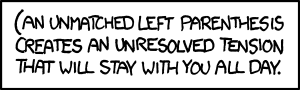
\includegraphics[scale=0.7]{xkcd/(.png}
		\vspace{-7pt}
		\caption{ \texttt{\url{https://xkcd.com/859/}} }
	\end{figure}
\end{frame}

\section{Dokumente}
\begin{frame}{Dokumente}
	\begin{itemize}
		\item Dokumente bestehend aus drei Aspekten
		\pause
		\item \textbf{Inhalt}: Was steht eigentlich da?
		\item \textbf{Struktur}: Wie ist der Text gegliedert/strukturiert?
		\item \textbf{Form}: Wie ist das Erscheinungsbild ?
	\end{itemize}
\end{frame}

\mycomment{
\section{Kontextfreie Grammatiken}
\begin{frame}{Kontextfreie Grammatiken}
	
	\begin{Definition}
		Eine \textbf{kontextfreie Grammatik} ist ein 4-Tupel $G = (N, T, S ,P)$ mit
		\begin{itemize}
			\item[$N$] Alphabet von Nichtterminalsymbolen
			\item[$T$] Alphabet von Terminalsymbolen ($N \cap T = \emptyset$)
			\item[$S$] Startsymbol ($S \in N$)
			\item[$P$] Produktionsmenge ($P \subseteq N \times (N \cup T)^\ast$)
		\end{itemize}
	\end{Definition}

	\pause
	\begin{Beispiel}
		Sei $A$ das deutsche Alphabet (mit Klein-/Großbuchstaben).\\
		$G_{MI} := \left(\{S, M, I, N\}, \, A \cup \N_+, \, S, \, P\right)$ mit
		\begin{align*}
			P = \{S &\to \text{M\word\sp I\word\sp N}, \\
			M &\to \word{Monkey}, \\
			I &\to \word{Island}, \\
			N &\to \word 1 \mid \word 2 \mid \word 3 \}
		\end{align*}
	\end{Beispiel}
\end{frame}

\begin{frame}{Kontextfreie Grammatiken}
	\begin{block}{Produktionen}
		$=$ Menge von Ersetzungsregeln. \\
		Schema: \\
		\qqquad $\underbrace{L}_{\mathclap{\text{\textbf{genau ein} Nichtterminal}}} \to [\text{rechte Seite aus \word{Terminalen} und/oder Nichtterminalen}]$ \\
		\smallskip
		Heißt: Wir können in \textbf{einem} Ersetzungsschritt \textbf{genau ein} solches Nichtterminal $L$ mit der rechten Seite ersetzen. \textbf{Wenn wir wollen}. \\
		\medskip
		\pause
		Mehrere Möglichkeiten zur Auswahl: \\
		\qquad $L \to [\text{rechte Seite}]_1 \mid [\text{rechte Seite}]_2 \mid [\text{rechte Seite}]_3 \mid ...$ \\
		Heißt: $L$ kann durch die rechte Seite 1, 2 oder 3 ersetzt werden. \textbf{Wie wir wollen.} \\
		\pause
		\begin{Beispiel}
			$S \to \word aB\word x \mid \word{zz}$ \\
			\impl $S$ kann durch $\word aB\word x$ oder \word{zz} ersetzt werden.
		\end{Beispiel}
	\end{block}
\end{frame}

\begin{frame}{Ableitungen von Wörtern}
	\begin{Definition}
		Wort $u = .....X.....$ \textbf{ableitbar} nach $v = ..... w......$ \\
		wenn es eine Produktion $X \to w$ gibt. \; ($X$ ist Nichtterminal.) \\
		Schreibweise: \quad $u \derives v$ \quad oder \quad $u \derives^1 v$ \\
	\end{Definition}
	
	\medskip
	\textbf{\alert{Achtung}}: Aufpassen mit Pfeilen: \quad  $\derives$ vs. $\to$
	
	\pause
	\begin{Beispiel}
		Für $G_{MI}$ gilt: \\
		$S \derives M\word{\sp} I\word{\sp}N$\\
		$ M\word{\sp} I\word{\sp}N \derives \word{Monkey}\word{\sp} I\word{\sp} N \derives \word{Monkey}\word{\sp} I\word{\sp 3}$ \\
		$\word{Monkey}\word{\sp} I\word{\sp} N \derives \word{Monkey}\word{\sp} I\word{\sp 1} \derives \word{Monkey}\word{\sp}\word{Island}\word{\sp 1}$ \\
		Es gibt kein Wort, das aus \word{Monkey\sp Island\sp 1} abgeleitet werden kann.
	\end{Beispiel}
	
\end{frame}

\begin{frame}{Ableitung}	
	\begin{block}{Schreibweisen}
		$u \derives^k v$ \quad heißt: $u$ in $k$ Schritten ableitbar zu $v$ \\
		$u \derives^0 v$ \quad heißt also: in 0 Schritten ableitbar ($u=v$) \\
		\smallskip
		$u \derives^* v$ \quad heißt: $u$ in \emph{beliebig vielen} Schritten ableitbar zu $v$
	\end{block}
	
	\mycomment{
		\pause
		\begin{block}{Beobachtung}
			Die Definitionen stimmen mit den Potenzen der Relation $\derives$ überein.\\
			$\derives^\ast$ ist die reflexiv-transitive Hülle von $\derives$.
		\end{block}
	}
	
	\pause
	\begin{Beispiel}
		Für $G_{MI}$ gilt: $S \derives^3 \word{Monkey\sp Island\sp}N \derives^1 \word{Monkey\sp Island\sp3}$\\
		$S \derives^* \word{Monkey\sp Island\sp2}$
	\end{Beispiel}
\end{frame}


\begin{frame}{Erzeugte Sprache einer Grammatik}
	\begin{Definition}
		Sei $G = (N, T, S, P)$ eine kontextfreie Grammatik. Wir nennen die Sprache $$L(G) := \{w \in T^\ast \mid S \Rightarrow^\ast w \} \subseteq T^*$$ die von $G$ \textbf{erzeugte Sprache}.
	\end{Definition} \pause
	Das sind also alle Wörter aus \emph{Terminalsymbolen}, die vom Startsymbol aus ableitbar sind.\\
	\bigskip
	Achtung: Die erzeugte Sprache kann auch \textbf{leer} sein. \\
	\§{Beispiele:} \pause $L\left(\left(\{X\},\, \{\word a, \word b\},\, X\, ,\{X\to X\}\right)\right) = \emptyset$ \pause \quad oder \\
	\. $L\left(\left(\{X\},\, \{\word a, \word b\},\, X\, ,\emptyset \right)\right) = \emptyset$
\end{frame}

\begin{frame}{Erzeugte Sprache}
	\begin{Beispiel}
		$L(G_{MI}) = \{\word{Monkey\sp Island\sp1}, \word{Monkey\sp Island\sp 2}, \word{Monkey\sp Island\sp 3}\}$\\
		$M\wordsp I\wordsp N \notin L(G_{MI})$ \quad (enthält nämlich  Nichtterminale!)
	\end{Beispiel}
	
	\pause
	\begin{Definition}
		Eine Sprache $L$, für die irgendeine kontextfreie Grammatik G mit $L(G) = L$ existiert, heißt \textbf{kontextfrei}.
	\end{Definition}
	\medskip
	
	Viele Programmiersprachen sind kontextfrei. \\  
	% ACHTUNG, streng genommen falsch. Jede Sprache, in der nur zuvor deklarierte Bezeichner als solche gültig sind, ist eigentlich kontext-sensitiv. Aber viele solcher Sprachen werden beim Parsen mittels einer kontextfreien Grammatik zerlegt; Deklariertheit von Bezeichnern wird dann später überprüft. Daher die allgemein für solche Sprachen gängige Bezeichnung „kontextfrei“.
	% Fun fact: Einrücksensitive Sprachen (wie Python – oder Haskell <3) sind dies streng genommen nicht! Das Lexing kann dann nicht von einem Regex-Automaten gemacht werden, der („übermächtige“ Stack-Automaten-)Lexer muss dann den Input vorverarbeiten, der daraus entstehende Tokenstream kann dann kontextfrei geparst werden.  Source: http://trevorjim.com/python-is-not-context-free/
	Eine vereinfachte Variante der englischen Sprache auch. \smiley
% Grob falsch:
%	Viele \enquote{natürlich vorkommende} Sprachen sind kontextfrei.
		
\end{frame}

%%%%%%%%%%%%%%%%%%%%
} % end mycomment
%%%%%%%%%%%%%%%%%%%%

\subsection{Beispiele}
\begin{frame}{Beispiel}
	$$ G = (\{X\}, \, \{\word a, \word  b\}, \, X, \, \{X \to \word aX\word b \mid \eps\}) $$
	\delimitershortfall=1pt
	\begin{itemize}
		\item Gilt $X \derives \word aX\word b$, \; $X \derives \word{aa}X\word{bb}$, \; $XX \derives \word{a}X\word{ba}X\word{b}$? \\
			  \visible<2-|handout:2->{Ja, Nein, Nein.}
		\item Welche Wörter über $\{\word a, \word  b\}$ lassen sich aus $\word{aa}X\word{bb}$ ableiten? Und aus $XX$? \\
			  \visible<3-|handout:2->{
				  Aus $\word{aa}X\word{bb}$: \quad $\set{\word a^k\word b^k \mid k \geq 2}$ \\
				  Aus $XX$: \quad $\set{\word a^k\word b^k \word a^\ell \word b^\ell \mid k,\ell \in \N_0}$
			  }
		\item Gebt $L(G)$ an! \\
		      \visible<4-|handout:2->{ $L(G) = \set{\word a^k\word b^k\mid k \in \N_0}$ }
	\end{itemize}
	
\end{frame}

\begin{frame}{Klammerausdrücke}
	Gegeben sei die Grammatik $$G = (\{X\}, \{\word{(}, \word)\}, X, \{X \to XX \mid \word(X\word) \mid \eps\})$$
	\begin{itemize}
		\item Wie leitet man \word{(())} ab?
		\item Wie leitet man \word{()()} ab?
		\item Kann man \word{(()(} ableiten? \pause \impl Nein!
		\item Und wie leitet man \word{(())()()} ab?\\ \pause
			$X \derives XX \derives XXX \derives \word(X\word)XX \derives \word(X\word)X\word(X\word) \derives \word(X\word)\word(X\word)\word(X\word)$ \\
			$\quad \derives \word(X\word{)()(}X\word) \derives \word{((}X\word{))()(}X\word) \derives \word{((}X\word{))()()} \derives \word{(())()()}$\\
			Geht das auch übersichtlicher? \impl Ableitungsbäume
	\end{itemize}
\end{frame}


\begin{frame}{Ableitungsbäume}
	\centering
	$G = (\{X\}, \{\word{(}, \word)\}, X, \{X \to XX \mid \word(X\word) \mid \eps\})$
	\medskip
	
	\begin{tikzpicture}
	[level 1/.style={sibling distance=50mm},
	level 2/.style={sibling distance=30mm},
	level 3/.style={sibling distance=10mm}]
	\node {$X$}
	child { node {$X$}
		[level 2/.style={sibling distance=15mm}]
		child {node {$\literal{(}$} }
		child {node {$X$} 
			child {node {$\literal{(}$} }
			child {node {$X$}
				child {node {$\varepsilon$} }
			}
			child {node {$\literal{)}$} }
		}
		child {node {$\literal{)}$} }
	} 
	child { node {$X$} 
		child { node {$X$} 
			child {node {$\literal{(}$} }
			child {node {$X$}
				child {node {$\varepsilon$} }
			}
			child {node {$\literal{)}$} }
		}
		child { node {$X$} 
			child {node {$\literal{(}$} }
			child {node {$X$}
				child {node {$\varepsilon$} }
			}
			child {node {$\literal{)}$} }
		}
	} ;
	\end{tikzpicture}
\end{frame}


\begin{frame}{Klammerausdrücke}
	Gegeben sei die Grammatik $$G = (\{X\}, \{\word{(}, \word)\}, X, \{X \to XX \mid \word(X\word) \mid \eps\})$$
	Was ist $L(G)$? Was kann man also aus $X$ ableiten?\\ \pause 
	Alle \enquote{\textit{wohlgeformten Klammerausdrücke}} \quad ($=$ alle, die Sinn machen).\\[1em]
	
	Was bedeutet wohlgeformt in diesem Kontext?\\ \pause
	$$\forall w \in L(G): N_{\word(}(w) = N_{\word)}(w)$$ 
	Reicht das? \pause \impl Notwendig, aber nicht hinreichend! 

\end{frame}

\begin{frame}{Klammerausdrücke}
	Wir dürfen eine Klammer erst schließen, \textit{nachdem} wir sie geöffnet haben.\\
	Also: Anzahl der schließenden Klammern darf nie größer als Anzahl der öffnenden Klammern sein! \pause \\[1em]
	\impl Für jedes Präfix $v$ von einem Wort $w \in L(G)$ gilt $$N_{\word(} (v) \geq N_{\word)} (v)$$ \pause
	
	\textbf{Achtung}: Grammatiken sind \textbf{nicht eindeutig}! Wir können zur gleichen Sprache mehrere verschiedene erzeugende Grammatiken finden. \\
	Alternative Grammatik für wohlgeformte Klammerausdrücke: \pause $$G = (\{X\}, \, \{\word (, \word )\}, \, X, \, \{X \to \word(X\word)X \mid \varepsilon\})$$
\end{frame}

\begin{frame}{Und jetzt ihr...}
	Gebt jeweils eine Grammatik über dem Alphabet $T = \{\word a, \word b\}$ an, die folgende Sprache erzeugt:
	\begin{itemize}
		\item Alle Wörter, in denen irgendwo das Teilwort $\word{baa}$ vorkommt.\\
		\visible<2-|handout:2>{
			$(\{X,Y\},T,X,P)$ mit $P=\{X \to Y\word{baa}Y, Y \to \word aY \mid \word bY \mid \varepsilon\}$
		}
		
		\item Alle Wörter, in denen $\word{ab}$ als Teilwort vorkommt oder kein $\word a$ enthalten ist. \\
		\visible<3-|handout:2>{
			$G = (\{X, Y\}, T, X, P)$ mit $P = \{X \to \word bX \mid Y\word{ab}Y \mid \varepsilon, Y \to \word aY \mid \word bY \mid \varepsilon\}$
		}
		
		\item Die Menge aller Wörter $w\in T^*$ mit der Eigenschaft, dass
		für alle Präfixe $v$ von $w$ gilt: $\setsize{N_{\word{a}}(v) - N_{\word{b}}(v)} \leq
		1$.\\
		\emph{Tipp}: Was für eine Struktur haben Wörter der Länge $2$, $4$, \dots? \\
		% $\{ab, ba\}^*$
		\visible<4-|handout:2>{
			$(\{X,Y\},T,X,P)$ mit $P=\{X \to \word{ab}X \mid \word{ba}X \mid \word a \mid \word b \mid \varepsilon\}$
		}
		
	\end{itemize}
\end{frame}


\begin{frame}{Aufgabe: Palindrome}
	\begin{itemize}
		\item Geben Sie eine kontextfreie Grammatik $$G = (N, \{\word a, \word b\}, S, P )$$ an, für die $L(G)$ die Menge aller Palindrome über dem Alphabet $\{\word a, \word b\}$ ist.
		\item Geben Sie eine Ableitung der Wörter \word{baaab} und \word{abaaaba} aus dem Startsymbol Ihrer Grammatik an.
		\item Beweisen Sie, dass Ihre Grammatik jedes Palindrom über dem Alphabet $\{\word a, \word b\}$ erzeugt.\\
		(\emph{Tipp}: Induktion: Wenn's für $n$ und $n+1$ gilt, dann gilt's auch für $n+2$.)
	\end{itemize}
\end{frame}

\begin{frame}{Lösung}
	Die Grammatik $$G = (\{S\}, \{\word a, \word b\}, S, P = \{S \to \word aS\word a \ | \ \word bS\word b \ | \ \word a \ | \ \word b \ | \ \varepsilon \})$$ erzeugt gerade die Menge der Palindrome. \pause Die Ableitungen der Wörter mit dieser Grammatik sind 
	$$S \derives \word bS\word b \derives \word{ba}S\word{ab} \derives \word{baaab}$$
	$$S \derives \word aS\word a \derives \word{ab}S\word{ba} \derives \word{aba}S\word{aba} \derives \word{abaaaba}$$
\end{frame}

\begin{frame}{Lösung}
	Sei $w$ ein Palindrom über $\{\word a,\word b\}$. Wir zeigen durch Induktion über $n = \size{w}$, dass alle Palindrome aus $S$ abgeleitet werden können. \pause
	\begin{block}{Induktionsanfang} \pause
		Für $n = 0$ ist das leere Wort $\varepsilon$ in einem Schritt aus $S$ ableitbar. \\
		Für $n=1$: Die einzigen Wörter aus $\{\word a,\word b\}^\ast$ der Länge 1 sind $\word a$ und $\word b$. Auch diese sind offensichtlich aus $S$ ableitbar.
	\end{block}
 	\pause
	\begin{block}{Induktionsvoraussetzung} \pause
		Für ein festes, aber beliebiges $n \in \N_0$ gilt, dass alle Palindrome der Länge $n$ und alle Palindrome der Länge $n + 1$ aus S abgeleitet werden können.
	\end{block}
\end{frame}

\begin{frame}{Lösung}
		\begin{block}{Induktionsschritt}
			Sei $w$ ein Palindrom der Länge $n + 2$. Das erste (und damit auch das letzte) Zeichen sei oBdA. ein $\word a$. Dann gibt es ein $w' \in \{\word a, \word b\}^\ast$, so dass $w = \word aw'\word a$ ist. Da $w$ ein Palindrom ist, muss auch $w'$ ein Palindrom sein. Weiterhin gilt $\size{w'} = n$. \pause Nach IV gibt es somit eine Ableitung $S \derives^\ast w'$. Somit gibt es die Ableitung $$S \derives \word aS\word a \overset{IV}{\derives^\ast} \word aw'\word a = w$$ und $w \in L(G)$ folgt. \pause Entsprechendes gilt, wenn das erste Zeichen von w ein \word b ist. \\
			Mit der IV haben wir also gezeigt, dass auch Palindrome der Länge $n+1$ und $n+2$ aus $S$ ableitbar sind.
	\end{block}

\end{frame}

\begin{frame}{Gibt es noch mehr?}
	Viele Sprachen in der Informatik sind kontextfrei.\\[1em]
	Was ist mit der Sprache $L_{vv} = \{v\word cv \mid v \in \{\word a,\word b\}^*\}$\\
	\smallskip
	\pause
	In der Vorlesung: Es gibt keine kontextfreie Grammatik, die $L_{vv}$ erzeugt.\\
	\medskip
	\pause
	Können wir die Sprache trotzdem irgendwie \enquote{verarbeiten}?
	
	\begin{block}{}
		\Large
		\centering
		Soon...\\[1em]
	\end{block}
\end{frame}


\mycomment{%maybe next tut
	\begin{frame}{Rückblick: Kontextfreie Grammatiken}
		\begin{itemize}[<+->]
			\item Ein Vier-Tupel: $G = (N, T, S, P)$
			\item[] z.B. $N=\left\{X,Y\right\}, T=\left\{\word{a}, \word{b}\right\}, S=X, P=\left\{X \to \word a Y, Y \to Y \mid \word b \right\}$
			\item Produktionen definieren Ersetzungen eines Nichtterminals mit Wörtern über $N \cup T$
			\item Wir wenden Produktionen in Ableitungsschritten an: $v \Rightarrow w, v \Rightarrow^* w$
			\item[] z.B. $X \derives \word a Y$, $Y \derives Y$, $Y \derives^{2020} Y$, $\word{aaa}Y\word{bbb} \derives \word{aaabbbb}$, $X \derives^2 \word{ab}$ oder $X \derives^\ast \word{ab}$
			\item $L(G)$ sind alle aus $S$ ableitbaren Wörter über $T$ (die also nur aus Terminalsymbolen bestehen)
		\end{itemize}
	\end{frame}
}
%\begin{frame}[t]{Wahr oder Falsch?}
%	\Socrative
%	Sei $G=(\{X,Y\},\, \{\word a, \word b\},\, X,\, P)$ eine kontextfreie Grammatik. \\
%	\FalseQuestion{Die Produktion $XY \to \word a$ könnte eine gültige Produktion sein.}
%	\FalseQuestion{Die Produktion $\word a \to XY$ könnte eine gültige Produktion sein.}
%	\TrueQuestionE{Die Produktion $X \to X\word aX$ könnte eine gültige Produktion sein.}{}
%	\TrueQuestionE{Wenn $X \to w$ eine gültige Produktion ist, dann gilt $X \derives^* w$.}{}
%	\FalseQuestionE{Wenn $X \derives^* w$ gilt, dann ist $X \to w$ eine Produktion in P.}{Sei $P=\{X \to XX \mid \word a\}$. Dann gilt $X \derives^* X\word a$, aber $X \to X\word a \notin P$.}
%\end{frame}


%
\thasse{
	\begin{frame}{}
		\begin{block} {Aussagenlogik}
			\begin{itemize}
				\item \enquote{Es regnet und alle Vögel sind grau.}
				\item atomar: \enquote{Es regnet.}, \enquote{ Alle Vögel sind grau.}
				\item Diese beiden Aussagen lassen sich ihrerseits nicht in weitere Teilaussagen zerlegen!
			\end{itemize}
		\end{block}
		
		\pause
		\begin{block} {Prädikatenlogik}	
			\begin{itemize}
				\item In der Prädikatenlogik werden atomare Aussagen hinsichtlich ihrer inneren Struktur untersucht und quantifiziert.
				\item \enquote{Alle Vögel sind grau}
				\item lässt sich in : \enquote{Alle Vögel}, \enquote{sind grau} zerlegen.
			\end{itemize}
			
		\end{block}
	\end{frame}
}

\section{Prädikatenlogik: Syntax}

\begin{frame}{Syntax}
	\begin{block}{Aufbau von prädikatenlogischen Formeln}
	\begin{itemize}[<+->]
		\item \textbf{Terme}: Liefern \enquote{Werte} (Zahlen, Wörter, whatever...); \\ 
		Aus Konstanten, Variablen und Funktionssymbolen zusammengesetzt.
		\item \textbf{Atomare Formeln}: Liefern Wahrheitswerte $\in \BB$; \\
		 Aus Termen und Relationssymbolen zusammengesetzt.
		\item \textbf{Prädikatenlogische Formeln}: aus atomaren Formeln und AL-Konnektiven sowie Quantoren ($\forall, \exists$) zusammengesetzt. 
	\end{itemize}
	\end{block}
\end{frame}

\begin{frame}{Terme}
	Bestehen aus... \\
	\medskip
	
	\textbf{Variablen} \, (endlich viele) \quad Alphabet $\VPL$ \\
	$\word{x}_i$ \quad $\word x, \word y, \word z$ \\
	Können in einer Formel beliebig verschiedene Werte annehmen \\
	\medskip \pause
	
	\textbf{Konstanten} \, (endlich viele) \quad Alphabet $\CPL$ \\
	$\word{c}_i$ \quad $\word c, \word d$ \\
	Konstanter Wert in der gesamten Formel \\
	\medskip \pause
	
	\textbf{Funktionen} \, (endlich viele) \quad Alphabet $\FPL$ \\
	$\word{f}_i$ \quad $\word f, \word g, \word h$ \\
	Liefern Werte für irgendwelche Eingaben (wie gewohnt) \\
	Jedes $\word{f}_i$ hat Stelligkeit $\ar(\word{f}_i) \in \N_+$ \quad „Wieviel Argumente $\word{f}_i$ nimmt“ {\small (Arität)} \\
	\smallskip \pause
	
	Beispiel: 
	\quad Funktionen $\word f$ mit $\ar(\word f) = 2$, \quad $\word g$ mit $\ar(\word g) = 1$. \\ \pause
	\quad OK: \qquad \word{f(x,y)} \qquad \word{g(c)} \qquad \word{g(f(x,c))} \\
	\quad Kaputt: \qquad \word{f(c)} \qquad \word{g(x,y,z)} \qquad \word{f(x,y} \qquad \word{f(x,,}
\end{frame}

\begin{frame}{Atomare Formeln}
	Zusammengesetzt aus... \\
	\medskip
	
	\textbf{Termen} (von eben) als Argumente in \\
	\medskip
	
	\textbf{Relationen} \, (endlich viele) \quad Alphabet $\RPL$  \\
	$\pleq$ und beliebige $\word R_i$ \quad $\word R, \word S$ \\
	Liefern Wahrheitswerte in $\BB = \set{\W, \F}$ \\
	Haben auch Stelligkeit $\ar(\word R_i) \in \N_+$ \\
	\medskip \pause
	
	Beispiele: \quad Relationen \word R mit $\ar(\word R) = 1$, \quad \word S mit $\ar(\word S) = 2$ \\
	\quad $\word x \pleq \word c$ \qquad $\word{g(x)} \pleq \word{g(y)}$ \qquad $\word{R(g(c))}$ \qquad $\word{S(x,f(x,y))}$
	\medskip \pause
	
	Relationen und Funktionen können \textbf{nur mit Termen} aufgerufen werden! \\
	\impl \quad \word{R(S(x,y))} \qquad \word{g(S(x))} \qquad $\word{R(x)} \pleq \word{S(x,y)}$ \qquad $\word x \pleq \word{(}\word y \pleq \word z\word{)}$ \\
	Alles \textbf{falsch}!
\end{frame}

\begin{frame}{Prädikatenlogische Formeln}
	Bestehen aus... \\
	\medskip
	
	\textbf{Atomaren Formeln} (von eben) \\
	\medskip
	
	\textbf{AL-Konnektiven} \\
	$\alnot, \aland, \alor, \alimpl$ und Klammern {\small (einsparbar)} \\
	Verknüpfen PL-Formeln \\
	\medskip \pause
	
	\textbf{Quantoren} \\
	$\plall$ All-Quantor \quad $\plexist$ Existenz-Quantor \\
	Verwendung: $\bleftBr\plall \word x_i \text{...Formel...}\brightBr$ \quad $\bleftBr\plexist \word x_i \text{...Formel...}\brightBr$ \\
	\impl NUR \textbf{Variablen} können quantifiziert werden! \\
	\medskip 
	
	Klammerregeln: Wie bei AL-Formeln; Quantoren binden stärker als alles andere.
	\bigskip \pause
	
	\textbf{Falsch}: \\
	$\bleftBr\plexist \word c \text{...Formel...}\brightBr$ mit $\word c \in \CPL$ \quad \word c keine Variable! \\
	$\bleftBr\plall \word x \word{:} \text{...Formel...}\brightBr$ \quad KEINE Doppelpunkte! \\
\end{frame}

\begin{frame}{Aufgabe: Syntaktische Fehler}
	Findet jeweils den syntaktischen Fehler in den folgenden prädikatenlogischen Formeln:
	\begin{itemize}
		\item $\plexists \word z \: \plka \word{c(z)} \plkz$\\
		\visible<2-|handout:2>{Konstanten (\word c) sind keine Relationen!}
		\item $\word{S(c)} \aland \word{T(d)} \alimpl \word{S(R(c,d))}$\\
		\visible<3-|handout:2>{Nur Terme als Argumente, keine Relationen (\word{R(c,d)}).}
		\item $\plall \plx \plall \ply \: \word{R(f(x,f(y)))}$\\
		\visible<4-|handout:2>{$\ar(\word f) = 1$ oder $\ar(\word f) = 2$, aber nicht beides gleichzeitig.}
		\item $\plall \plx \: \plka \word{S(x)} \aland \word{T(x)} \plkz \alimpl \plexists \word R \: \plka \plall \plx \: \word{R(x,x)} \plkz $\\
		\visible<5-|handout:2>{Relationen können nicht quantifiziert werden ($\plexists \word R$).}
		\item $\plall \word f \: \word{S(f)} \aland \plall \plx \: \word{g(R(x))}$\\
		\visible<6-|handout:2>{Nur Terme als Argumente, keine Relationen (\word{R(x)}).\\
		Hinweis: $\plall \word f \: \word{S(f)}$ ist \emph{erlaubt}. Hier ist $\word f$ nur eine Variable, \word f muss nicht immer eine Funktion sein. Hier wird nirgends \word f „aufgerufen“ (\word{f(}...\word{)}).}
	\end{itemize}
\end{frame}

\begin{frame}{Formeln aufstellen}
	\begin{Beispiel}
		Alle Menschen lieben Weihnachten.\\ % Aber Gänse eher nicht...
		\medskip
		
		\pause
		$\plall \plx \; {\plka \word{Mensch(x)} \alimpl \word{liebt(x,Weihnachten)} \plkz}$
	\end{Beispiel}
% TODO: Zweites Beispiel (evtl. aus Übung klauen)
\end{frame}

\begin{frame}{Aufgabe 2 (WS 15/16, Blatt 7)}
	\begin{block}{Aufgabe}
		Formuliert die folgenden Aussagen als Formeln in Prädikatenlogik:
		\begin{enumerate}
			\item Nicht alle Vögel können fliegen.
			\item Wenn es irgendjemand kann, dann kann es Donald Ervin Knuth.
			\item John liebt jeden, der sich nicht selbst liebt.
		\end{enumerate}
	\end{block}
	
	\visible<2-|handout:2>{
		\begin{block}{Lösung}
			\begin{enumerate}
				\item \qqquad $\plexist \plx {\plka \plfoo{Vogel}{\plka \plx \plkz} \aland \alnot \plfoo{flugfähig}{\plka \plx \plkz} \plkz}$
				\visible<3-|handout:2>{
					\item \qqquad $
					\plexist \plx {\plka \plfoo{kann\_es}{\plka \plx \plkz} \plkz}
					\alimpl
					\plfoo{kann\_es}{\plka \plfoo{knuth} \plkz}
					$
				}
				\visible<4-|handout:2>{
					\item \qqquad $
					\plall \plx {\plka \alnot \plfoo{liebt}{\plka \plx \plcomma \plx \plkz} \alimpl \plfoo{liebt}{\plka \plfoo{John} \plcomma \plx \plkz} \plkz}
					$
				}
			\end{enumerate}
		\end{block}
	}
\end{frame}

\begin{frame}{Freie und gebundene Variablenvorkommen}
	\textbf{Vorkommen} einer Variable in einer PL-Formel: \\
	$G = \plall \word{x\,R(\underline{x})}$ \Impl \word x kommt in $G$ vor. \\
	„Direkt hinter Quantoren“ zählt nicht! \\
	Bsp.: $F = \plall \word{x\,R(c)}$ \Impl \word x kommt \textbf{nicht} in $F$ vor! \\
	\medskip \pause
	
	\textbf{Freie Variablenvorkommen} \quad $\fv(F)$ \\
	Alle, die \emph{irgendwo} in $F$ vorkommen, ohne dass sie quantifiziert sind {\small ($=$ ein Quantor sie einführt)}. \\
	\smallskip \pause
	Beispiel: $\fv\left(\word{R(\underline{x},\underline{y},c)} \aland \plexist \word x\, \plka \word x \pleq \underline{\word y} \plkz \right) = \set{\word x, \word y}$ \\
	\medskip \pause
	
	\textbf{Gebundene Variablenvorkommen} \quad $\bv(F)$ \\
	Alle, die \emph{irgendwo} in $F$ vorkommen und dabei quantifziert sind. \\
	\smallskip \pause
	Beispiel: $\bv\left(\word{R(x,y,c)} \aland \plexist \word x\, \plka \underline{\word x} \pleq \word y \plkz \right) = \set{\word x}$ \\
	\medskip \pause
	
	Formel $F$ heißt \textbf{geschlossen} $:\!\!\Gdw \fv(F) = \emptyset$\\
	\medskip 

\end{frame}

\begin{frame}{Freie und gebundene Variablenvorkommen}
	\begin{equation*}
	F = \plexist \plx \, \plE{\plka \plx \plcomma \ply \plkz}
		\, \alor \,
		\plall \plz \, \plall \plx \, \plall \ply \, {\plka
			\plE{\plka \plx \plcomma \plz \plkz} \aland \plE{\plka \ply \plcomma \plz \plkz}
		\plkz}
	\end{equation*}
	
	\begin{block}{Aufgabe}
		Welche Variablenvorkommen sind frei ($\fv$) und welche gebunden ($\bv$)?\\
		Ist die Formel geschlossen?
	\end{block}

	\pause
	\begin{block}{Lösung}
		Nur die Variable $\fv(F) = \{\ply\}$ kommt frei in $F$ vor.\\
		Genau die Variablen $\bv(F) = \{\plx, \ply, \plz\}$ kommen gebunden in $F$ vor.\\
		Da $\fv(F) \neq \emptyset$, ist $F$ nicht geschlossen.
	\end{block}
	
\end{frame}

\begin{frame}{Substitutionen}
	\delimitershortfall=0pt
	Wollen \textbf{Variablen} (!) durch andere Terme ersetzen. \\
	\impl Eine Substitutionsabbildung $$\sigma_S \from \LFor \functionto \LFor, \quad \text{längliche Definition s. VL}$$ wendet Ersetzungen aus $S$ auf eine Formel an. \\
	\medskip \pause
	
	Beispiel: \\
	$\sigma_{\set{\word x/\word y}}\left(\word x \pleq \word c\right) = \word y \pleq \word c$. \\
	$\sigma_{\set{\word x/\word{f(c)}}}\left(\word{R(x,y)} \aland \plexists  \word y\,\plka\word y \pleq \word x \plkz\right) = \word{R(\word{f(c)},y)} \aland \plexists  \word y\,\plka\word y \pleq \word{f(c)\plkz}$. \\
	\medskip \pause
	
	Mehrere auf einmal: \\
	$\sigma_{\set{\word x/\word y, \, \word y/\word x}}\left(\word x \pleq \word y\right) = \word y \pleq \word x$.
\end{frame}

\begin{frame}{Substitutionen}
	\delimitershortfall=0pt
	Ersetzt werden nur \textbf{freie Variablenvorkommen}!\\
	Gebundene Vorkommen, also Variablen im Wirkungsbereich eines (eigenen) Quantors, werden \textbf{nicht} ersetzt. \\
	\medskip \pause
	
	Beispiel: \\
	$\sigma_{\set{\word y/\word{f(c)}}}\left(\word{R(x,y)} \aland \plexists \word y\, \plka\word y \pleq \word x \plkz\right) = \word{R(x,\word{f(c)})} \aland \plexists \word y\,\plka\word y \pleq \word x \plkz$
	
\end{frame}

\begin{frame}{Substitutionen: Kollisionsfreiheit}
	Bei einer \textbf{kollisionsfreien} Substitution werden keine Variablen durch Ersetzung \enquote{aus Versehen} gebunden.  \\
	\medskip
	Ersetzen wir eine freie Variable $\word x$ durch einen Term, in dem die Variable $\word y$ frei vorkommt, so darf sich $\word x$ nicht im Wirkungsbereich eines Quantors über $\word y$ befinden. \\
	(Sonst wird \word y nämlich unfreiwillig quantifiziert und die Bedeutung ändert sich!)
	
	\pause
	\begin{Beispiel}
		$F = \plall \plx \plka\plx \pleq \ply\plkz$\\
		Kollisionsfrei: $\sigma_{\{\ply/\plz\}}(\plall \plx \plka\plx \pleq \ply\plkz) = \plall \plx \plka\plx \pleq \underline{\plz}\plkz$\\
		Nicht kollisionsfrei: $\sigma_{\{\ply/\plx\}}(\plall \plx \plka\plx \pleq \ply\plkz) = \plall \plx \plka\plx \pleq \underline{\plx}\plkz$ 
	\end{Beispiel}
\end{frame}

\begin{frame}{Substitutionen: Aufgabe}
	$F = \alnot \plexist \plx {\plka \plE{\plka \plx \plcomma \ply \plkz}\plkz}$\\
	$G = \plall \plx \plall \ply {\plka 
			\plE{\plka \plx \plcomma \plz \plkz} \aland 
			\plE{\plka \ply \plcomma \plz \plkz} \plkz}$
	\medskip
	
	Gebt jeweils eine Substitution $\sigma$ an, die \emph{nicht} kollisionsfrei für $F$ bzw. $G$ ist.\\[1em] \pause
		
	\impl Die Substitution $\sigma_{\{\ply/\plx\}}$ macht $F$ kaputt.\\ \pause
	\impl Die Substitutionen $\sigma_{\{\plz/\plx\}}$ oder $\sigma_{\{\plz/\ply\}}$ machen $G$ kaputt.
	
\end{frame}



%\input{../Bloecke/Praedikatenlogik2}

\begin{frame}	
	\begin{block}{Was ihr nun wissen solltet}
		\begin{itemize}
			\item Was kontextfreie Grammatiken sind
			\item Wie man Sprachen mit Grammatiken beschreiben kann
			\item Wie man Grammatiken arbeiten kann
			%\item Welche Eigenschaften Relationen haben können
			%\item Wie Prädikatenlogische Formeln aufgebaut sind
			%\item Wie man damit präzise Aussagen trifft
			%\item Wie man sie auswertet
		\end{itemize}
	\end{block}
	
	\begin{block}{Was nächstes Mal kommt}
		\begin{itemize}
			\item Weitere Eigenschaften von Relationen
			\item Wie Prädikatenlogische Formeln aufgebaut sind
			\item Wie man prädikatenlogische Formeln auswertet
			\item Wie man damit präzise Aussagen trifft
		\end{itemize}
	\end{block}
\end{frame}

%\begin{frame}[plain]
%	\begin{center}
%		\large
%		Nicht vergessen, Kinder: Nächste Woche findet noch ein Tutorium statt! \smiley
%	\end{center}
%\mycomment{	\bigskip
%	Für alle die nicht kommen: \\
%	Frohe Weihnachten und einen guten Start in das neue Jahr!}
%\end{frame}

\xkcdframe{704}{Danke für eure Aufmerksamkeit! \smiley}{2.5}
%\lastframe{0.50}{0}{xkcd/logic_principle_of_explosion.png}{https://www.xkcd.com/}
%\lastframe{0.50}{0}{xkcd/christmastree.png}{https://www.xkcd.com/835} % Dieses Jahr dürften noch genügend Tutanden beim nächsten Termin kommen
\slideThanks

\end{document}